\documentclass[acmtoms,acmnow]{acmtrans2m}
%\documentclass[a4paper]{paper}
\usepackage{graphicx}
\usepackage{amssymb}
\usepackage{amsmath,amsfonts}
\usepackage{xtab}


%\newtheorem{theorem}{Theorem}[section]
%\newtheorem{conjecture}[theorem]{Conjecture}
%\newtheorem{corollary}[theorem]{Corollary}
%\newtheorem{proposition}[theorem]{Proposition}
%\newtheorem{lemma}[theorem]{Lemma}
%\newdef{definition}[theorem]{Definition}
%\newdef{remark}[theorem]{Remark}


\begin{document}

\begin{center}
{\Huge LMEF Manual}\\[5mm]
{\Large D.S. Vlachos  and T.E. Simos}\\[5mm]
{\Large University of Peloponnese}\\[5mm]
e-mail: \texttt{dvlachos@uop.gr, simos@uop.gr}
\end{center}

\vspace{1cm} % 1 cm vertical spacing


%\markboth{Vlachos et al.}{LMEF Manual }

\begin{abstract}
LMEF is a program written in MATLAB, to calculate the coefficients of a linear multi-step method (explicit, implicit or backward differentiation formulas) with algebraic and/or exponential fitting for the numerical solution of first order ordinary differential equations. Moreover, LMEF calculates the local truncation error and in the case of exponential fitting, the Taylor expansions of the coefficients which are necessary for the implementation of the method.
\end{abstract}


%\maketitle

\section{Introduction}
LMEF is a MATLAB program that calculates the coefficients of a linear multi-step method with exponential fitting. A linear multistep method is of the form:
\begin{equation}
\sum_{j=0}^{k}a_j y_{n-j} -h\sum_{j=0}^{k}b_jy'_{n-j}=0
\end{equation}
There are three types of methods that are handled by LMEF. The first one is explicit methods, in which the user gives the $a$-coefficients and the program calculates the $b$'s, assuming that $b_0=0$. The second type is implicit methods in which again the user gives the $a$-coefficients and the program calculates the $b$'s. Finaly, the third type is $BDF$ methods in which the user just gives the number of steps and the program calculates the $a$-coefficients. 
The syntax of LMEF is:
\begin{verbatim}
[c,ct,r]=lmef(e_i , a , q , t);
\end{verbatim}
where

\begin{xtabular}{p{0.1\textwidth}p{0.8\textwidth}}
{\it e\_i} & is either $'e'$ for explicit methods, $'i'$ for implicit ones or $'b'$ for backward differentiation formulas (BDF methods are implicit but as it was explained before, $'i'$ for LMEF means that the program it is asked to calculate the $b$-coefficients given the $a$-coefficients, while $'b'$ means that the program is asked to calculate the $a$-coefficients of a BDF method). 
\\
{\it a} & is a column vector containing the values of the coefficients $a$'s \\
{\it q} & is a row vector containing information about the number of the frequencies to be fitted. The value $1$ means that the method must integrate exactly the term $e^{qx}$ while the value $2$ means that the method must integrate exactly the functions $e^{\pm q x}$ \\
{\it t} & is a row vector containing the level of tuning for each given frequency.
\end{xtabular}

The output values are:

\begin{xtabular}{p{0.1\textwidth}p{0.8\textwidth}}
{\it c} & is a vector containing all the coefficients, both the given and the calculated ones in the form $(a_0,...,a_k,b_0,...,b_k)^T$
 \\
{\it ct} & is a vector containing the Taylor expansions of the coefficients $c$'s
\\
{\it r} & is the reminder of the method.
\end{xtabular}

If only the first two parameters are given, then algebraic fitting is assumed. If the vector containing the level of tuning is missing, then simple fitting is assumed (level of tuning equals to $0$).

Both Taylor expansions of the coefficients $c$'s and calculation of the residual of the method require either MATLAB build-in functions or external functions from MAPLE {\it like mtaylor} which may fail to compute the expansion especially in multiple frequency fitting although the limit of the expression under expansion always exists (when frequencies or step size tends to zero). To solve this problem, a function called {\it my\_mtaylor} has been developed which separates the numerator and denominator of the expression under expansion, calculates the Taylor expansions of those two new expressions and finally calculates the Taylor expansion of their quotient. It can be easily proved that the expansion calculated in this way is exact up to the minimum order of expansion of the nominator and denominator. 

In the case of backward differentiation formulas, the values of the given a-coefficients are neglected and only the dimension of the a-vector is used (the number of steps). 

LMEF performs some basic tests on the input parameters in the case of explicit or implicit methods. Using the coefficients $a$, it calculates the roots of the characteristic polynomial of the method and checks the following:
\begin{itemize}
\item $1$ must be a root of the characteristic polynomial. 
\item The roots must lie in the unit disc, and those that lie on the unit circle must have multiplicity one, otherwise an error message is displayed and the calculations stop.
\end{itemize}


\section{Customization}
In the first lines of LMEF, there are some variables that can be altered by the user. These are:
\begin{itemize}
 \item \textit{te\_order}: the order up to which Taylor expansions of the coefficients are calculated. The default value is $10$.
\item \textit{rc\_order}: a root $r$ is considered to lie in the unit disc if $|r|<1+rc\_order$. The default value is $10^{-5}$.
\end{itemize}

\section{Test Run}
\subsection{Algebraic fitting}
Consider the method
\begin{equation}
y_n-y_{n-1}=h\left(b_0y'_{n}+b_1y'_{n-1}+b_2y'_{n-2}+b_3y'_{n-3}\right)
\nonumber
\end{equation}
The call to LMEF is as follows:
\begin{verbatim}
>>[c,ct,e]=lmef('i',[1,-1,0,0]');
\end{verbatim}
We can see now the coefficients $c$'s and the residual of the
method:
\begin{verbatim}
>> disp(c)
     1
    -1
     0
     0
   3/8
 19/24
 -5/24
  1/24
>> disp(e)
-19/720*y_5*h^5
\end{verbatim}
where $y\_5$ is a way to represent $y^{(5)}(x)$ and $h^{\wedge} 5$
means $h^5$.

\subsection{Simple exponential fitting part 1}
Consider the same method as in A1 but now the method must
integrate exactly the function $e^{qx}$. The call to LMEF is as
follows:
\begin{verbatim}
>> [c,ct,e]=lmef('i',[1,-1,0,0]',[1]);
\end{verbatim}
We can see now, for example, $b_0$ and the Taylor expansion of
$b_0$ which in the c-vector is $c(5)$:
\begin{verbatim}
>> pretty(c(5))
  1/12 (12 exp(3/2 q_1 h~) + 16 q_1 h~ exp(- 1/2 q_1 h~)
         - 23 q_1 h~ exp(1/2 q_1 h~) - 12 exp(1/2 q_1 h~)
         - 5 q_1 h~ exp(- 3/2 q_1 h~))/(q_1 h~ (3 exp(- 1/2 q_1 h~)
         - 3 exp(1/2 q_1 h~) - exp(- 3/2 q_1 h~) + exp(3/2 q_1 h~)))
>> disp(ct(5));
3/8-19/720*q_1*h-1/180*q_1^2*h^2+1/12096*q_1^3*h^3+...
\end{verbatim}
and finally the residual
\begin{verbatim}
>> disp(e);
19/720*(-y_5+y_4*q_1)*h^5
\end{verbatim}
In the above expressions, $y\_n$ represents $y^{(n)}$ and $q\_1$
the frequency. We can easily verify that both the coefficients
$c$'s and the residual of the method tend to the classical values
calculated in A1 when $q\_1 \rightarrow 0$:
\begin{verbatim}
>> syms q_1
>> limit(e,q_1,0)
ans =

-19/720*y_5*h^5


>> limit(c,q_1,0)
ans =

     1
    -1
     0
     0
   3/8
 19/24
 -5/24
  1/24
\end{verbatim}

\subsection{Simple exponential fitting part 2}
Again as in A2 but now the functions $e^{\pm qx}$ must be fitted.
The call to LMEF is as follows:
\begin{verbatim}
>> [c,ct,e]=lmef('i',[1,-1,0,0]',[2]);
\end{verbatim}
The Taylor expansion of $b_0$ is ($c(5)$:
\begin{verbatim}
>> disp(ct(5));
3/8-3/160*q_1^2*h^2+3/2240*q_1^4*h^4-31/268800*q_1^6*h^6+...
\end{verbatim}
The residual of the method is:
\begin{verbatim}
>> disp(e);
19/720*(-y_5+y_3*q_1^2)*h^5
\end{verbatim}
Again we can check the values of the coefficients $c$'s and the
residual when $q\_1\rightarrow 0$.
\begin{verbatim}
>> syms q_1
>> limit(c,q_1,0)
ans =

     1
    -1
     0
     0
   3/8
 19/24
 -5/24
  1/24

>> limit(e,q_1,0)
ans =

-19/720*y_5*h^5
\end{verbatim}

\subsection{Exponential fitting with level of tuning greater than 0}
Again as in A3 but know, the functions $e^{\pm qx}$ and $xe^{\pm
qx}$ must be fitted. The call to LMEF is as follows:
\begin{verbatim}
>> [c,ct,e]=lmef('i',[1,-1,0,0]',[2],[1]);
\end{verbatim}
The Taylor expansion of $b_0$ and the residual are:
\begin{verbatim}
>> disp(ct(5));
3/8-3/80*q_1^2*h^2+5/896*q_1^4*h^4-113/134400*q_1^6*h^6+...

>> disp(e);
-19/720*(y_5+y_1*q_1^4-2*y_3*q_1^2)*h^5
\end{verbatim}
Again, the limit of the coefficients $c$'s and the residual, when
$q\_1 \rightarrow 0$ are:
\begin{verbatim}
>> syms q_1
>> limit(c,q_1,0)
ans =

     1
    -1
     0
     0
   3/8
 19/24
 -5/24
  1/24

>> limit(e,q_1,0)
ans =

-19/720*y_5*h^5
\end{verbatim}

\subsection{Exponential fitting with two frequencies}
Again as in A1 but know, the functions $e^{\pm q_1 x}$ and $e^{\pm
q_2 x}$ must be fitted. The call to LMEF is as follows:
\begin{verbatim}
>> [c,ct,e]=lmef('i',[1,-1,0,0]',[2,2]);
\end{verbatim}
The Taylor expansion of $b_0$ and the residual are:
\begin{verbatim}
>> disp(ct(5));
3/8+(-3/160*q_1^2-3/160*q_2^2)*h^2+
(-43/4480*q_1^2*q_2^2-11/2240*q_2^4-11/2240*q_1^4+1/53222400*
(11/20*q_1^2+11/20*q_2^2)*(604800*q_1^2+604800*q_2^2))*h^4+...

>> disp(e);
-19/720*(y_1*q_1^2*q_2^2-q_1^2*y_3-y_3*q_2^2+y_5)*h^5
\end{verbatim}
Again the limit of the coefficients $c$'s and the residual when
both $q\_1,q\_2 \rightarrow 0$ are:
\begin{verbatim}
>> syms q_1 q_2
>> limit(limit(b,q_1,0),q_2,0)
ans =

     1
    -1
     0
     0
   3/8
 19/24
 -5/24
  1/24

>> limit(limit(e,q_1,0),q_2,0)
ans =

-19/720*y_5*h^5
\end{verbatim}

\subsection{Backward Differentiation Formula with Algebraic Fitting}
Consider now the formula
\begin{equation}
\sum_{j=0}^{4}a_jy_{n-j}=h\cdot y'_n
\end{equation}
We can calculate the a-coefficients by calling lmef:
\begin{verbatim}
>> [c,ct,e]=lmef('b',[1 1 1 1 1]');
\end{verbatim}
The coefficients are:
\begin{verbatim}
>> c

c =

 25/12
    -4
     3
  -4/3
   1/4
     1
     0
     0
     0
     0
\end{verbatim}
and the truncation error
\begin{verbatim}
>> e

e =

-1/5*y_5*h^5
\end{verbatim}

\subsection{Backward Differentiation Formula with Exponential Fitting}
Consider again the formula of A.6 but now we want the method
to be trigonometrically fitted. Then
\begin{verbatim}
>> [c,ct,e]=lmef('b',[1 1 1 1 1]',[2]);
\end{verbatim}
Then, the Taylor expansion of $a_0$ is:
\begin{verbatim}
>> ct(1)

ans =

25/12+1/6*q_1^2*h^2-5/72*q_1^4*h^4+25/864*q_1^6*h^6-
    125/10368*q_1^8*h^8+625/124416*q_1^10*h^10...
\end{verbatim}
and the truncation error
\begin{verbatim}
>> e

e =

1/5*(y_3*q_1^2-y_5)*h^5
\end{verbatim}
Again, it is easily verified that in the case of $q\_1\rightarrow 0$
we get the method of A.6.

\section{Testing the constructed methods}
In order to test the constructed methods, we provide the program \textit{wrapping.m}. Function <<wrapping>> tests a linear multistep method. Call the function:
\begin{verbatim}
>>wrapping(c,problem,h,N)
\end{verbatim}
where
\begin{itemize}
 \item \textit{'c'} are the coefficients of the method in symbolic form [a,b] 
\item \textit{'problem'} i a handle to the function f, such that $y'(t)=f(t,y(t))$. The detailed communication protocol with this function is the following:
\begin{itemize}
\item Call problem(0,0,1) to display a message
\item Call problem(h,k,2) to calculate the first k-values with step size -h
\item Call problem(Y,n\_omega,3) to calculate a set of n\_omega frequencies given the current value Y
\item Call problem(Y,t,4) to calculate the Jacobian given the current value Y and the current time -t
\item Call problem(t,Y) to calculate the derivative at time -t given Y=Y(t)
\end{itemize}
\item \textit{'h'} is the integration step
\item \textit{'N'} is the iterations number
\end{itemize}
The output is:
\begin{itemize}
 \item Y, the values of the calculated function. The value at position -i-, corresponds to t=(i-1)*h
\item T, a vector with the times at which Y is calculated
\end{itemize}

\subsection{Test problem}
As a test example, we calculate the motion of two bodies in a reference system that is fixed in one of them. Moreover, the motion is planar, thus, we only have to calculate the $x$ and $y$ coordinates of the second body. The differential equations are:
\begin{eqnarray}
 \ddot{x}=&&-\frac{x}{\sqrt{x^2+y^2}^3} \nonumber \\
 \ddot{y}=&&-\frac{y}{\sqrt{x^2+y^2}^3} \nonumber 
\end{eqnarray}
and the initial conditions are
\begin{eqnarray}
 x(0)=1-\epsilon & \dot{x}(0)=0 \nonumber \\
y(0)=0 & \dot{y}(0)=\sqrt{\frac{1+\epsilon}{1-\epsilon}} \nonumber
\end{eqnarray}
where $\epsilon$ is the eccentricity. By setting $y_1=x$, $y_2=y$, $y_3-y_1'$ and $y_4=y_2'$, we get the first order system:
\begin{equation}
\left( \begin{array}{l}y_1 \\ y_2 \\ y_3 \\ y_4 \end{array}\right)'=\left( \begin{array}{l} y_3 \\ y_4 \\ -\frac{y_1}{\sqrt{y_1^2+y_2^2}^3} \\ -\frac{y_2}{\sqrt{y_1^2+y_2^2}^3} \end{array} \right)
\end{equation}

In the first case (low eccentricity $=0.2$) we consider the explicit method $EM-4$:
\begin{verbatim}
[c,ct,e]=lmef('e',[1,-1,1,-1]');
\end{verbatim}
and the method $EM-4_{TF}$ with trigonometric fitting:
\begin{verbatim}
[c_o,ct_o,e_o]=lmef('e',[1,-1,1,-1]',[2]);
\end{verbatim}
The detailed sequence of MATLAB commands is:
\begin{verbatim}
>>[c,ct,e]=lmef('e',[1,-1,1,-1]');
>>[c_o,ct_o,e_o]=lmef('e',[1,-1,1,-1]',[2]);
>>f_02(0.2,0,5);% set the eccentricity to 0.2
>>[Y_,T_]=wrapping(c,@f_02,0.075,1500);
>>t=subs(c_o,'q_1','sqrt(-1)*q_1');
>>[Y_o,T_o]=wrapping(t,@f_02,0.075,1500);
>>plot(Y_(:,1),Y(:,2),'g');
>>hold on
>>plot(Y_o(:,1),Y_o(:,2),'r');
\end{verbatim}

Figure \ref{fig_res_EM_4} presents the calculated position of the second body using methods $EM-4$ and $EM-4_{EF}$ using step size $h=0.075$ for $112,5$ periods. The relative error in energy, momentum and angular momentum is also shown. The effect of trigonometric fitting is obvious from this figure.

In the second case (high eccentricity $=0.75$) we consider the explicit method $EM-7$:
\begin{verbatim}
[c,ct,e]=lmef('e',[1,-1,1,0,-1,1,-1]');
\end{verbatim}
the method $EM-7_{TF}$ with trigonometric fitting:
\begin{verbatim}
[c_o,ct_o,e_o]=lmef('e',[1,-1,1,0,-1,1,-1]',[2]);
\end{verbatim}
and the BDF method $BDF-5$:
\begin{verbatim}
[c_b,ct_b,e_b]=lmef('b',[1,1,1,1,1]');
\end{verbatim}
The detailed sequence of MATLAB commands is:
\begin{verbatim}
>>[c,ct,e]=lmef('e',[1,-1,1,0,-1,1,-1]');
>>[c_o,ct_o,e_o]=lmef('e',[1,-1,1,0,-1,1,-1]',[2]);
>>[c_b,ct_b,e_b]=lmef('b',[1,1,1,1,1]');
>>f_02(0.75,0,5);% set the eccentricity to 0.75
>>[Y_,T_]=wrapping(c,@f_02,0.01,750);
>>t=subs(c_o,'q_1','sqrt(-1)*q_1');
>>[Y_o,T_o]=wrapping(t,@f_02,0.01,750);
>>[Y_b,T_b]=wrapping(c_b,@f_02,0.001,750);
>>plot(Y_(:,1),Y(:,2),'g');
>>hold on
>>plot(Y_o(:,1),Y_o(:,2),'b');
>>plot(Y_b(:,1),Y_b(:,2),'r');
\end{verbatim}

Figure \ref{fig_res_EM_7} presents the calculated position of the second body using methods $EM-7$, $EM-7_{TF}$ and $BDF-5$ with step size $h=0.01$ for $7,5 periods$. Simple trigonometric fitting cannot stabilize the solution, although the implicit BDF method keeps the second body on the expected orbit.

\clearpage
\begin{figure}
\begin{center}
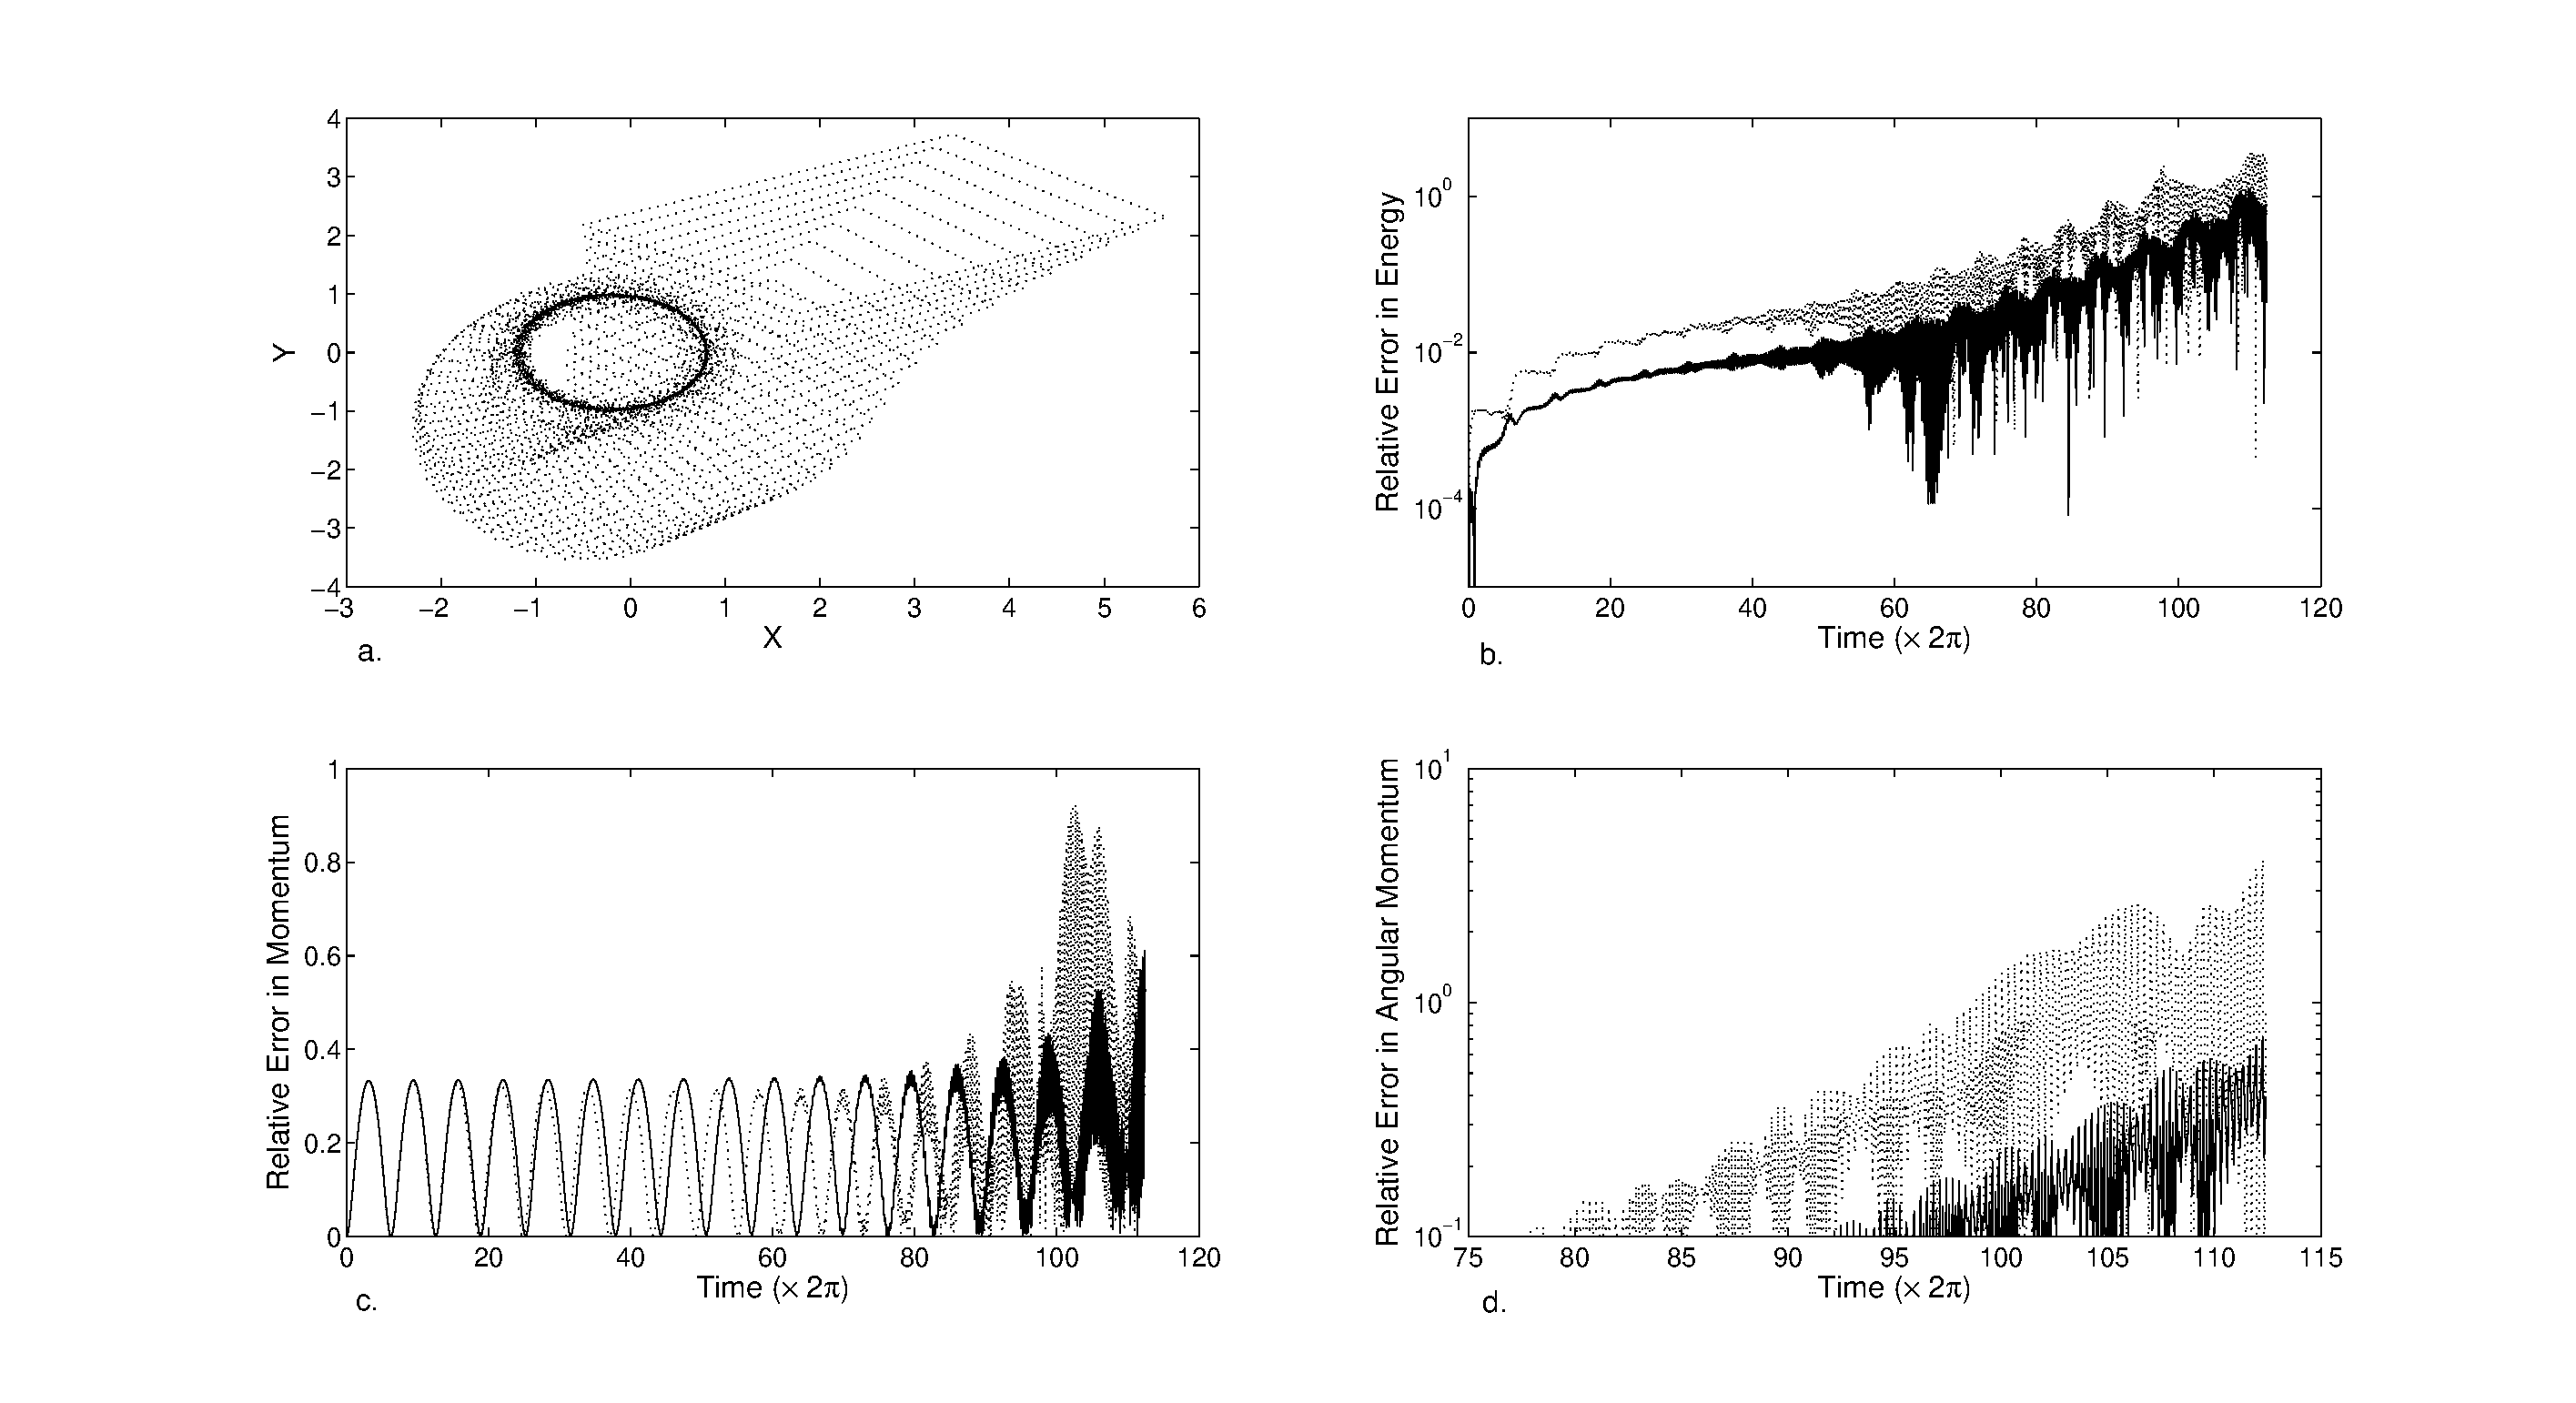
\includegraphics[width=15cm]{2bp_e_2_ME_4.eps}
\caption{Integration of the 2-body problem for eccentricity $\epsilon=0.2$, step size $h=0.075$ for $112.5$ periods. (a) The calculated position of the second body using methods $EM-4$ (dotted line) and $EM-4_{TF}$ (solid line), (b) the relative error in energy for the method $EM-4$ (dotted line) and $EM-4_{TF}$ (solid line), (c) the relative error in momentum for the method $EM-4$ (dotted line) and $EM-4_{TF}$ (solid line) and (d) the relative error in angular momentum for the method $EM-4$ (dotted line) and $EM-4_{TF}$ (solid line).} \label{fig_res_EM_4}
\end{center}
\end{figure}

\clearpage
\begin{figure}
\begin{center}
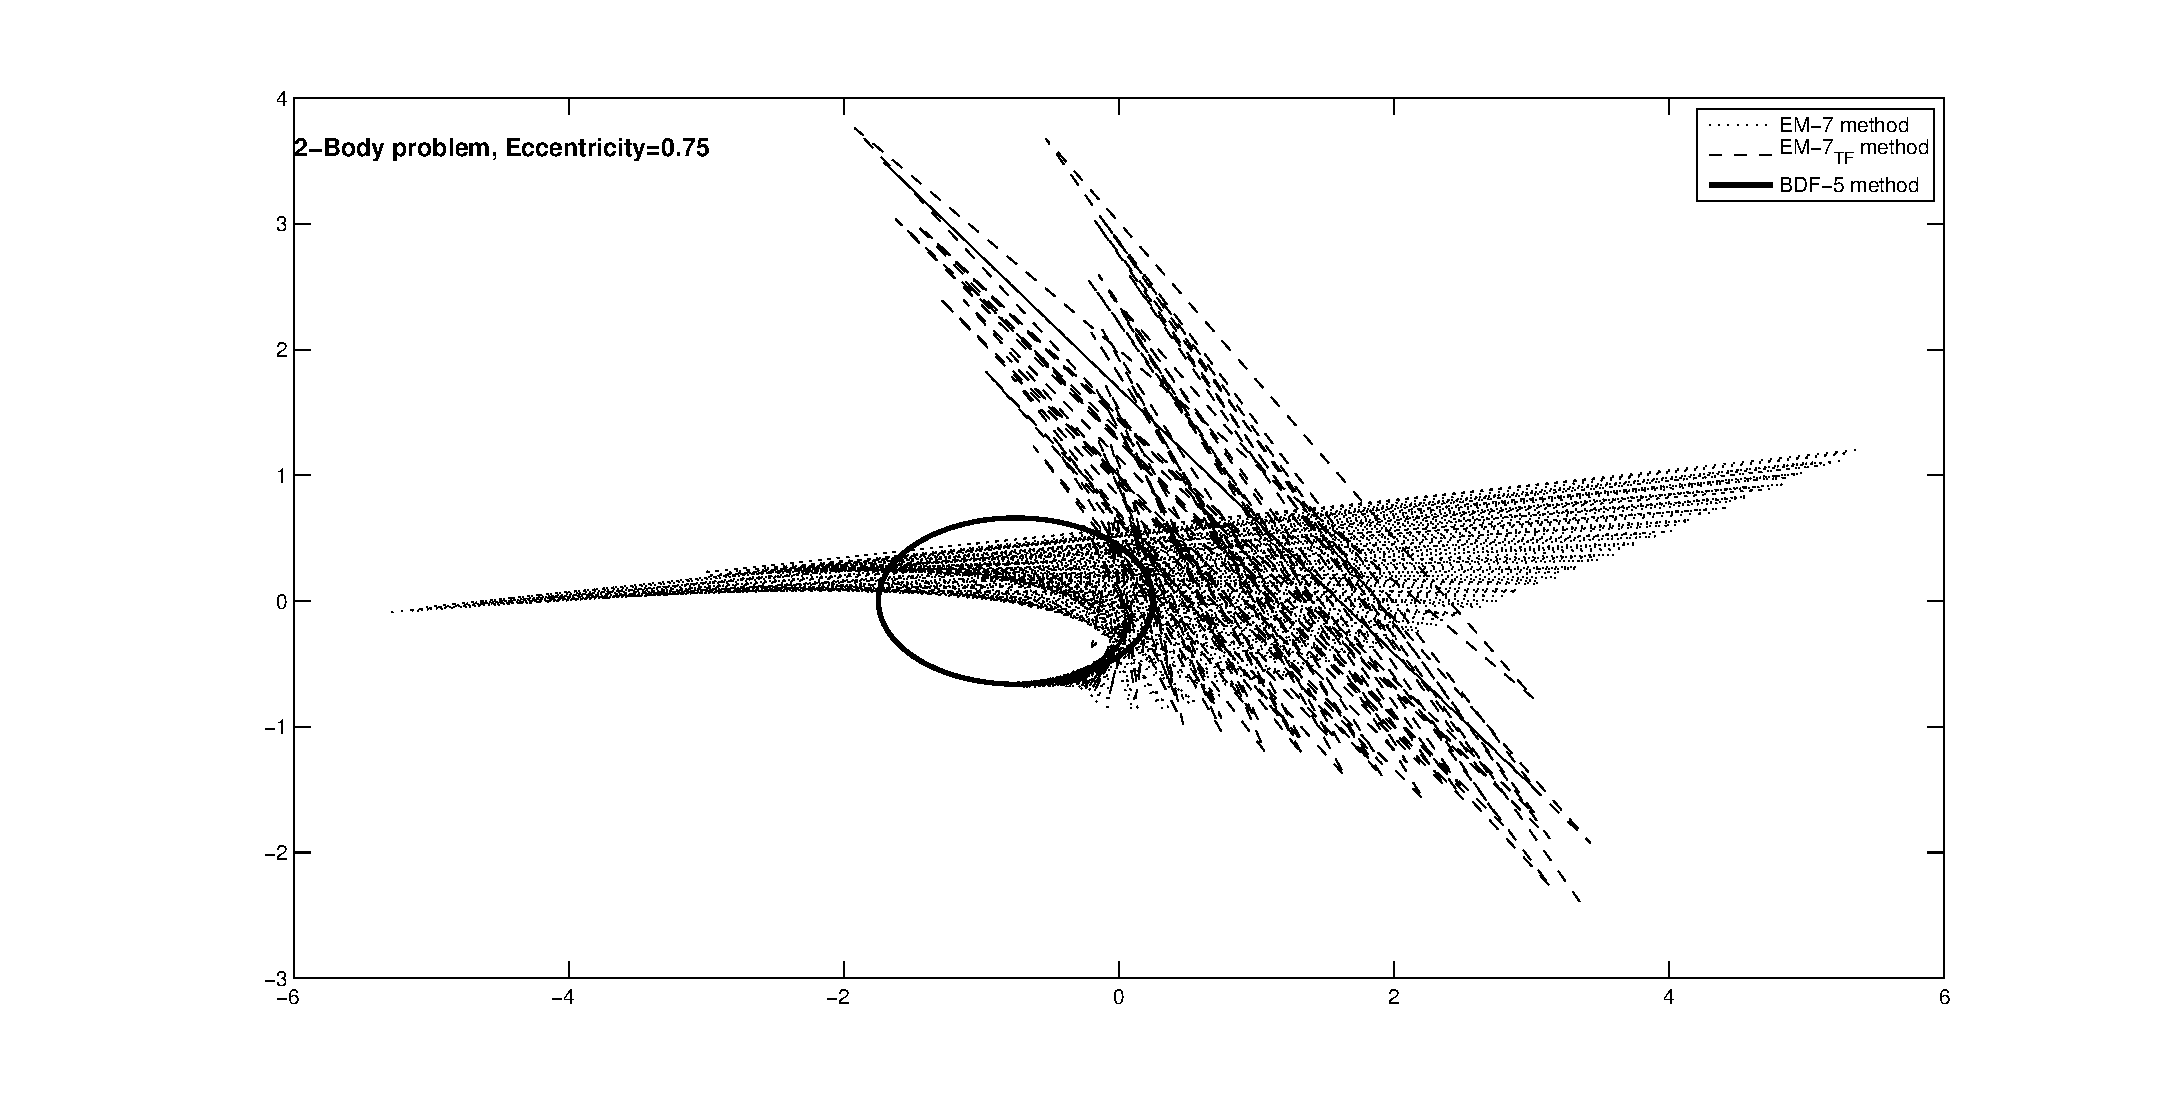
\includegraphics[width=15cm]{2bp_e_75_ME_7_BDF_5.eps}
\caption{The calculated position of the second body using methods $EM-7$ (dotted line), $EM-7_{TF}$ (dashed line) and $BM-5$ (solid line) with step size $h=0.01$ for $7,5 periods$.} \label{fig_res_EM_7}
\end{center}
\end{figure}

\end{document}
